\documentclass{article}
\usepackage[spanish]{babel}
\usepackage[numbers,sort&compress]{natbib}
\usepackage[T1]{fontenc}
\usepackage[ansinew]{inputenc}
\usepackage{graphicx}
\usepackage{url}
\usepackage{caption}
\usepackage{float}
\usepackage{subcaption}
\usepackage{caption}
\usepackage{listings}
\usepackage{amsmath}
\usepackage{natbib}



\title {Interacciones entre part\'iculas}
\author{Oscar Qui\~nonez}

\begin{document}

\maketitle
 
\section{Objetivo}\label{met}

En el presente trabajo se realiza la simulaci\'on de un conjunto de part\'iculas que interact\'uan entre ellos a trav\'es de las fuerzas de atracci\'on y repulsi\'on que ejercen sobre ellas las cargas pertenecientes a cada part\'icula. As\'i tambi\'en se simula el efecto de la gravedad y las masas para conocer la manera en que se distribuye la velocidad de estas part\'iculas. 

\section{Metodolog\'ia}\label{met}

Para llevar a cabo la simulaci\'on, fue necesario el uso del programa Python 3.7, donde se colocaron 60 part\'iculas a las que se les atribuy\'o una carga el\'ectrica aleatoria con valores entre -1 y 1, si dos part\'iculas ten\'ian la misma carga se ejerc\'ia una repulsi\'on, y si hab\'ia una carga diferente se presentaba una atracci\'on \cite{satuelisa}. Del mismo modo se atribuy\'o una masa aleatoria a las part\'iculas para representar la forma en la que la gravedad las afectaba, todo esto en un periodo de 200 pasos; se us\'o como c\'odigo base \cite{doctora} el anteriormente proporcionado en clase.

\section{Resultados y Discusi\'on}\label{res}

Al t\'ermino de la ejecuci\'on del c\'odigo se obtuvieron 2 tipos de gr\'aficas: de dispersi\'on, en el que se observan las posiciones de las part\'iculas y el movimiento que realizan debido a las fuerzas de atracci\'on y repulsi\'on que existen entre ellas (ver figura 1) ; y un grupo de histogramas que representan la manera en la que se distribuyen las velocidades con respecto al valor de las cargas que poseen las part\'iculas, se puede apreciar que en el rango de -0.80 a -0.65 la distribuci\'on fue nula y entre -0.20 y 0 se obtuvo la mayor parte de esta (ver figura 2). As\'i tambi\'en se observan en las gr\'aficas la distribuci\'on de las masas (ver figura 3) donde la mayor\'ia de las part\'iculas poseen un valor entre -0.6 y 1.1; adem\'as de los promedios de las velocidades (ver figura 4) donde se puede ver que el rango m\'as destacado se encuentra entre 0.91 y 1.

\begin{figure}
       \centering
       \begin{subfigure}[b]{0.49\linewidth}
           \includegraphics[width=\linewidth]{tareanueve_t0.png}
           \caption{Paso 0}
           \label{fig:westminster_lateral}
        \end{subfigure}
        \begin{subfigure}[b]{0.49\linewidth}
            \includegraphics[width=\linewidth]{tareanueve_t040.png}
            \caption{Paso 40}
            \label{fig:westminster_aerea}
        \end{subfigure}
        \begin{subfigure}[b]{0.49\linewidth}
            \includegraphics[width=\linewidth]{tareanueve_t080.png}
            \caption{Paso 80}
            \label{fig:westminster_aerea}
        \end{subfigure}
        \begin{subfigure}[b]{0.49\linewidth}
            \includegraphics[width=\linewidth]{tareanueve_t120.png}
            \caption{Paso 120}
            \label{fig:westminster_aerea}
        \end{subfigure}
        \begin{subfigure}[b]{0.49\linewidth}
            \includegraphics[width=\linewidth]{tareanueve_t160.png}
            \caption{Paso 160}
            \label{fig:westminster_aerea}
        \end{subfigure}
        \begin{subfigure}[b]{0.49\linewidth}
            \includegraphics[width=\linewidth]{tareanueve_t200.png}
            \caption{Paso 200}
            \label{fig:westminster_aerea}
        \end{subfigure}
        \caption{Posiciones de las part\'iculas en incrementos lineales de 40 hasta llegar a 200.}
        \label{fig:westminster}
\end{figure}

\begin{figure}
  \centering
  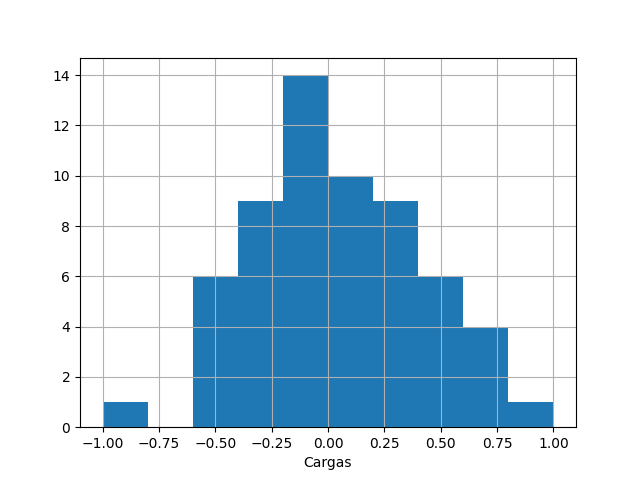
\includegraphics[scale=0.85]{tareanuevecargas.png}
  \caption{Distribuci\'on de las cargas}
  \label{fig2}
\end{figure}

\begin{figure}
  \centering
  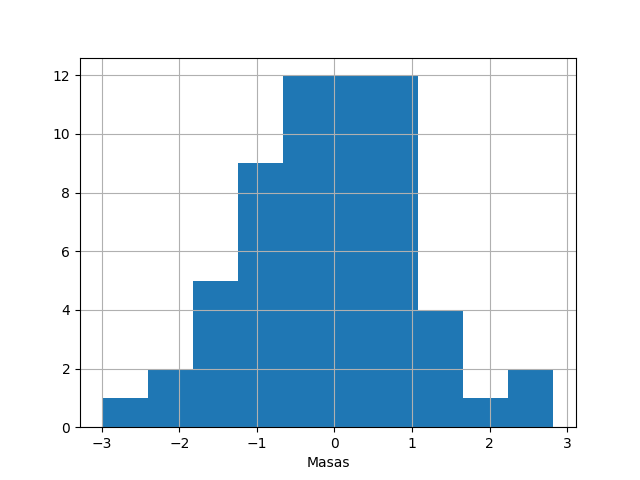
\includegraphics[scale=0.85]{tareanuevemasas.png}
  \caption{Distribic\'on de las masas}
  \label{fig3}
\end{figure}

\begin{figure}
  \centering
  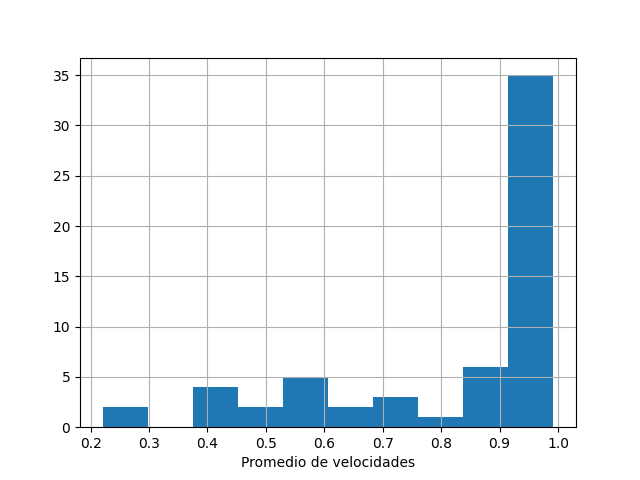
\includegraphics[scale=0.85]{tareanuevepromedio.png}
  \caption{Distribic\'on de velocidades}
  \label{fig4}
\end{figure}

\newpage
\section{Conclusi\'on}

Se pudo observar como el comportamiento de las part\'iculas se ve afectado de acuerdo a los par\'ametros que le agregamos en la simulaci\'on, las masas de las part\'iculas estaban distribuidas de manera similar entre cargas positivas y negativas, mientras que en el promedio de las velocidades si se ve\'ia una distribuci\'on muy marcada entre los valores mas altos con respecto a los mas bajos, por su parte las cargas estaban distribuidas de manera equitativa, 30 con valores negativos y 30 con valores positivos. En el apartado correspondiente \cite{yo} se encontrar\'a con una imagen en formato GIF de la gr\'afica de dispersi\'on para los 200 pasos simulados.

\bibliography{tareanueve}
\bibliographystyle{unsrtnat}

\end{document}
